\documentclass{article}
\usepackage[usenames]{color} %used for font color
\usepackage{amssymb} %maths
\usepackage{amsmath} %maths
\usepackage[utf8]{inputenc} %useful to type directly diacritic characters
%\usepackage[linesnumbered,ruled,vlined]{algorithm2e}
\addtolength{\topmargin}{-.975in}
%\pagenumbering{gobble}
\usepackage{url}
%\usepackage{hyperref}
\usepackage{float}
\usepackage{pgfplots}
\usepackage{tikz}
\usepackage{graphicx}
\usepackage[french]{babel}



\title{Premier Rapport INF6404A : Couches Dispositifs et Réseaux}
\author{
	Alexandre Mao\\
	David Johannès \\
	Philippe Troclet \\
	Fabien Berquez \\
	D\'{e}partement G\'{e}nie Informatique et G\'{e}nie Logiciel \\
	\'{E}cole Polytechnique de Montr\'{e}al, Qu\'{e}bec, Canada \\
	\texttt{alexandre.mao@polymtl.ca}\\
	\texttt{david.johannes@polymtl.ca}\\
	\texttt{philippe.troclet@polymtl.ca}   \\
	\texttt{fabien.berquez@polymtl.ca}   \\
}
\date{11 mai 2016}

\usepackage{natbib}
\usepackage{graphicx}

\begin{document}

\maketitle

\section{Introduction}

Le progrès établi dans les domaines scientifiques et technologiques a permis l’apparition et le développement de nouveaux objets, similaires à ceux que nous connaissons actuellement, mais avec la faculté supplémentaire d’être connectés à Internet. Ce déploiement d’Internet aux objets physiques est appelé Internet Of Things, ou IoT.

IoT représente donc une nouvelle manière de voir notre monde d’aujourd'hui, à savoir un monde où les objets communiquent entre eux, et sont interconnectés. Plus précisément, IoT est un « réseau de réseaux qui permet, via des systèmes d’identification électronique normalisés et sans fil, d’identifier et de communiquer numériquement avec des objets physiques afin de pouvoir mesurer et échanger des données entre les mondes physiques et virtuels » \cite{benghozi2009internet}
\\

Bien évidemment, IoT a vu le jour afin de répondre à des problématiques importantes, notamment avoir la possibilité de fournir une mesure en continue de certaines variables, tout en minimisant les coûts technologiques, de maintenance, et en ressources humaines.
\\

L’IoT peut ainsi être appliqué au Smart Health, à savoir être utilisé dans les soins cliniques où les patients, dont le statut physiologique nécessite une attention particulière, peuvent être surveillés en permanence en utilisant des outils de surveillance non invasifs et dirigés par l’IoT. Cela nécessite par conséquent des capteurs sans fils pour recueillir de l'information physiologique précise et complète, et implique d’utiliser des passerelles (gateways) et le Cloud pour analyser et stocker les informations, puis pour envoyer (de manière sans fil) les données analysées aux aides-soignants et aux médecins pour une analyse et des examens plus approfondis.

Ces techniques permettraient d’améliorer la qualité des soins grâce à une surveillance constante et de réduire le coût des soins en éliminant la nécessité d’avoir activement et systématiquement un aide-soignant pour collecter et analyser les données.

En outre, la technologie peut être utilisée pour la surveillance à distance à l'aide de petites solutions connectées sans fil à travers l'IoT. Ces solutions peuvent être utilisées pour capturer des données en toute sécurité sur la santé des patients à partir d'une variété de capteurs, pour appliquer des algorithmes complexes pour analyser les données, puis pour les partager grâce à la connectivité sans fil avec les professionnels médicaux qui peuvent faire des recommandations de soins appropriées.

Il faut donc permettre aux applications de surveillance de santé de collecter des données provenant de capteurs, de fournir un support pour les interfaces et les affichages de l’utilisateur, d’avoir une connexion au réseau pour l’accès aux services de l’infrastructure, et bien évidemment d’être robuste, durable, précis, fiable, et faible en consommation d’énergie \cite{vermesan2014internet}.
\\

Pour en revenir aux objectifs principaux de tels hôpitaux « intelligents », ils se résument à améliorer la qualité de vie des personnes qui ont besoin de surveillance permanente, à diminuer les barrières concernant la surveillance d’importants paramètres de santé, à éviter les coûts et les efforts de santé inutiles, et à fournir un support médical juste et approprié au bon moment.
\\

Dans le cadre de nos laboratoires, nous nous intéresserons donc aux hôpitaux, et plus particulièrement aux services de soins intensifs qui nécessitent une surveillance permanente de patients (qu’ils soient animés ou inanimés, et l’utilisation de hautes technologies de mesure. Le but de nos laboratoires sera alors d’apporter une solution IoT face à la congestion des hôpitaux, et plus précisément dans les services de soins intensifs, en distinguant plusieurs cas d’utilisation (patients inanimés ou non). Notre premier laboratoire consistera à décrire les différents dispositifs qu’il est possible d’utiliser dans notre cas, ainsi que les protocoles de réseau et de communication qu’il faudra appliquer pour permettre à nos dispositifs de communiquer entre eux. Aussi, nous établirons en dernier lieu les problématiques liées à notre solution. 

\section{Les Dispositifs}

 Les hôpitaux fournissent à la population un service essentiel et vital, cependant de nombreux problèmes se présentent à eux. Ils peuvent faire face à de fortes demandes pendant toute la journée ce qui peut amener à une congestion au niveau du traitement des patients lors des fortes affluences dans certains départements. L’un des défis important que rencontre les hôpitaux est donc la gestion de ces périodes de fortes affluences qui passe par la gestion de son personnel et l’optimisation du service qu’il fournit. Et dans certains départements, le personnel médical doit être omniprésent auprès des patients pour un suivi de l’évolution des cas les plus critiques, ce qui a pour conséquence un besoin de personnel plus important et ainsi un sur-coût important pour l’hôpital.
 
 Nous allons nous intéresser dans notre cas, à un département de l’hôpital qui requiert une forte présence humaine et une attention très importante dans sa gestion. Ce département est celui des soins intensifs :
 
 « Les unités de soins intensifs (ou USI) sont des services hospitaliers spécialisés dans la prise en charge des patients inanimés ou particulièrement malades nécessitant une surveillance permanente. De manière générale, les services de soins intensifs ont pour mission de maintenir en vie des patients en état critique dont le pronostic vital est engagé dans la mesure où leurs fonctions vitales sont affectées. En soins intensifs, les malades sont surveillés par des équipes spécialisées disposant d'un matériel de haute technicité. » \cite{SoinsIntensifs}

Le système que nous allons proposer va avoir pour but de surveiller l’état des patients de manière continue et de telle sorte à ce que ces informations soient transmises rapidement au personnel médical et permettent ainsi un suivi de l’évolution de la santé du patient plus facile. Le système que nous proposons a pour but d’optimiser le temps passé par le personnel médical auprès du patient et de s’occuper de surveiller certaines fonctions vitales et environnementales du patient tout en permettant d’indiquer au personnel médical toute anomalie détectée. Il a aussi pour but de réduire les erreurs médicales liées aux fautes humaines. 

Nous présentons dans ce qui suit un ensemble d’appareils connectés destinés à surveiller le patient lors de sa présence dans les unités de soins intensifs jusqu'à sa sortie de celui-ci (transition d’un service à un autre par exemple) en fournissant un ensemble de capteurs et d’autre dispositifs pour permettre ce suivi lors de son séjour à l’hôpital. On décrira donc dans un premier temps les différents dispositifs nécessaires pour surveiller le patient et son environnement (les diverses conditions de sa chambre). Une telle mise en place de ces dispositif est illustrée sur la Figure 1. Les capteurs spécifiques représentent les capteurs qui ne sont appropriés que pour certains cas particuliers d’état du patient (coma, diabète, blessure grave, cancer).

\begin{figure}[h!]
	\hspace*{-3cm}
	\centering
	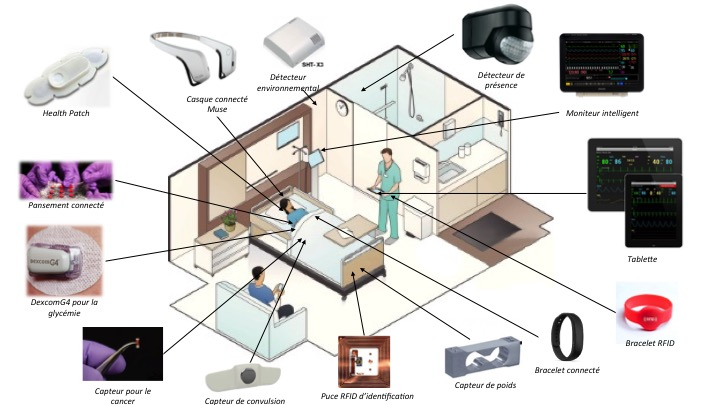
\includegraphics[width=1.5\textwidth]{Figure1.jpg}
	\caption{Dispositifs dans la Chambre du Patient}
	\label{fig:balance}
\end{figure}

On décrira ensuite les dispositifs nécessaires à mettre en place sut le patient pour le surveiller lors de son passage du service de soins intensifs à un autre service, et jusqu’à sa sortie de l’hôpital. Cette situation est illustrée par la Figure 2. En effet, une fois les soins intensifs terminés, il est nécessaire de continuer à surveiller le patient encore quelques temps avant de lui permettre de sortir de l’hôpital.
\\
\begin{figure}[h!]
	\hspace*{-1cm}
	\centering
	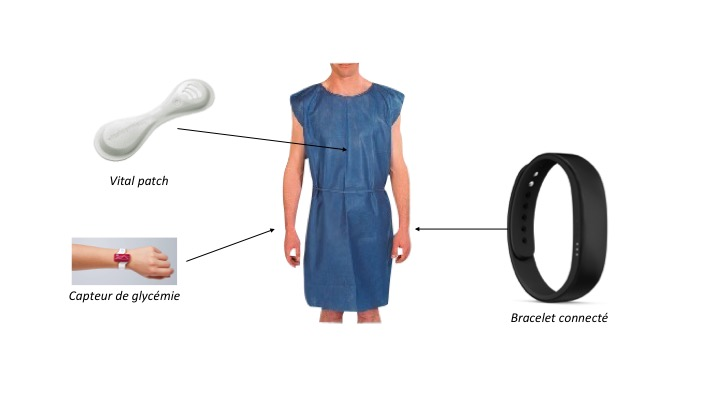
\includegraphics[width=1.2\textwidth]{Figure2.jpg}
	\caption{Dispositifs pour un patient classique}
	\label{fig:balance}
\end{figure}

Tout d’abord, afin de mesurer la fréquence respiratoire, le rythme cardiaque, la température du corps, la pression sanguine, et les phases de sommeil du patient, des capteurs peuvent être utilisés. Dans notre recherche des technologies IoT actuelles, il s’avère que le patch Health Patch \cite{HealthPatch} permet de mesurer toutes ces variables, ce qui a l’avantage de regrouper plusieurs capteurs en un seul élément  et ici sur un seul patch. On a besoin d’une mesure de ces variables en temps réel (surtout pour la fréquence respiratoire et le rythme cardiaque), et à chaque instant, ou pour être plus précis à chaque demi seconde, pour être rapidement prévenu en cas d’anomalie et afin de permettre au personnel soignant d’intervenir rapidement en cas d’urgence.

Pour les patients souffrant de cancer et subissant un traitement approprié, il est intéressant de pouvoir mesurer l’efficacité du traitement. Ainsi, il est intéressant de pouvoir utiliser un capteur qui permet de suivre l’évolution d’un cancer \cite{Cancer}, et qui est à placer au cœur de la tumeur. Grâce à un système de communication sans fil, le capteur récolte des informations sur la tumeur, à savoir : sa concentration en oxygène et son acidité. Il envoie ces informations en temps réel à un récepteur. Ces deux informations vont permettre aux médecins de savoir si le traitement administré au patient fonctionne ou non. En effet, si la tumeur s’acidifie de plus en plus, alors le traitement marche. Une hausse du taux d’oxygène est aussi un bon indicateur car elle révèle que la tumeur ne peut pas se développer (celle-ci se développant dans un milieu faible en oxygène). Il n’est pas nécessaire de relever les informations très fréquemment, étant donné la faible évolutivité d’une tumeur. Par conséquent, une mesure de ces variables toutes les 15 minutes est suffisante.

Certains patients en soins intensifs peuvent souffrir de diabètes. Il est donc nécessaire de pouvoir mesurer le taux de glycémie dans le corps du patient. Alphabet a développé le DexCom \cite{Diabete} qui  est un pansement connecté permettant justement de mesurer le taux de glycémie à travers la peau. Il possède l’avantage de ne pas piquer le patient pour effectuer cette mesure. Il pourra ainsi aider le personnel soignant à administrer les quantités d’insuline appropriée. Au niveau de la fréquence de la mesure du taux de glycémie, une collecte d’informations chaque minutes est suffisante, car le taux de glycémie peut varier modérément dans le temps.

Un autre de nos objectifs pour améliorer l’efficacité et la qualité de la surveillance du patient est de permettre d’avoir des capteurs qui puissent évaluer la cicatrisation de diverses blessures. Un pansement connecté futuriste et autonome \cite{Pansement}, qui est un pansement flexible et présentant une adhésion parfaite, semble idéal car le matériau qu’il intègre lui permet de coller fortement à plusieurs types de matériaux. Ainsi, il est possible d’intégrer des capteurs à l’intérieur du pansement, qui est utilisé à la surface de la peau du patient, et ces capteurs permettent de vérifier l’état des blessures et l’évolution de la cicatrisation. Une mesure toutes les 10 minutes est suffisante, car une blessure cicatrise assez lentement dans le temps.

Aussi, il est fréquent de recevoir dans le service des soins intensifs des patients inanimés ou dans le coma. Il devient alors nécessaire de mesurer et de surveiller en continu, c’est-à-dire toutes les demi secondes, l’activité cérébrale de ces patients. Un capteur peut alors être mise en place pour suivre l’activité cérébrale du patient. Nous avons vu l’exemple du casque Muse \cite{Muse}, qui « utilise des capteurs pour identifier les ondes générées par l’activité du cerveau. Les algorithmes de Muse détectent les changements subtils dans le cerveau et montrent l’activité en temps réel ». Cependant, ce dispositif est utilisé actuellement pour le divertissement. On suppose alors qu’un tel type de capteur peut exister à des fins médicales.

Une autre variable qui pourrait intéresser le médecin est le poids du patient tout au long de son séjour à l’hôpital. C’est pourquoi un capteur de force, placé au niveau du lit, et permettant de relever le poids du patient régulièrement, serait utile. Il ne suffirait cependant de relever le poids du patient que toutes les 12 heures, étant donné que cette variable évolue très peu d’un jour à l'autre (dans des conditions normales d'alimentation).

Afin de vérifier à n’importe quel moment où se situe le patient, il est important de pouvoir permettre sa localisation et traçabilité \cite{Localisation} assez fréquemment (toutes les 5 secondes, étant donné que le patient va passer une grande partie de son séjour dans le lit), à l’aide d’un bracelet qui serait placé au niveau de son poignet. 

Nous pouvons aussi voir si le patient peut présenter des convulsions, avec un capteur \cite{Convulsion} qui peut être posé pour mesurer les mouvements du patients toutes les secondes (ce capteur déclencherait une alarme s’il relève une trop forte variabilité du mouvement du patient sur une petite période). 

Il serait possible également de placer des capteurs de présence dans la chambre et les diverses pièces de la zone du patient (salle de bain, toilettes) afin de détecter la présence d’un patient dans ces pièces et le localiser dans sa zone. Ces capteurs n’auraient besoin de relever les données que toutes les 5 secondes, étant donné que l’on considère que le patient va se déplacer lentement tout au long de son séjour. Cela permettrait aussi à l’hôpital de connaître en quasi-temps réel l’occupation de ces chambres.

Tous les dispositifs décrits jusqu’à présent doivent être reliés à un moniteur principal intelligent, qui réunit toutes les informations de ces dispositifs pour les relayer au serveur de l’hôpital, mais qui également agit sur la perfusion possiblement reliée au patient afin d’administrer automatiquement et précisément un certain traitement, qui dépend des informations que le moniteur collecte. Par exemple, en collectant des informations sur le taux de glycémie du patient, le moniteur pourrait contrôler l’injection d’insuline nécessaire pour la santé du patient.

Une puce RFID (Radio Frequency Identification) \cite{RFID} pourrait également être placé au pied du lit du patient par exemple afin de permettre au médecin qui vient dans la chambre de pouvoir le scanner pour un accès rapide au dossier du patient. La puce RFID sera mise à jour fois qu’elle sera présente d’un lecteur RFID qui lui enverra les nouvelles données s’il y a eu des modifications.

Le but étant aussi de surveiller l’environnement du patient assez régulièrement (toutes les minutes) afin de lui procurer les meilleures conditions possibles, il faudrait pour cela placer des capteurs d’humidité, de température, de luminosité, \cite{HTL} et de fumée. 
\\

Lorsque le patient change de services, ou bien sort tout simplement du service de soins intensifs, il est nécessaire de surveiller encore certaines variables, pour vérifier que son état de santé est normal, et ce jusqu’à sa sortie de l’hôpital. 

Pour cela, il est nécessaire de maintenir la mesure de la fréquence respiratoire, du rythme cardiaque, de la température du corps, et de la pression sanguine, à savoir avoir un dispositif similaire à Health Path qui fournit ces mesures chaque demi seconde. D’après les technologies actuelles, Vital Patch \cite{VitalPatch}, qui se base sur la même technologie que Health Patch, propose de fournir ces mesures, et est approprié pour cette situation où le patient se déplace plus régulièrement dans l’hôpital.

Aussi, si le patient est diabétique, le même capteur de glycémie que précédemment (DexCom) peut être maintenu pour avoir une mesure régulière (toutes les minutes) du taux de glucose du patient.

Enfin, afin de permettre de localiser approximativement le patient, mais aussi permettre aux médecins d’avoir accès au dossier du patient, un bracelet muni d’une puce RFID (avec l’architecture appropriée pour proposer la localisation et les données du patient) peut être placé au poignet du patient. Ainsi, nous aurions des capteurs RFID disséminés un peu partout dans l’hôpital pour détecter les capteurs RFID des patients, et ainsi les localiser. Plus précisément, les capteurs RFID seront placés un peu partout dans les couloirs de l’hôpital, et à l’entrée de chaque chambre.
\\

Il est à noter, du côté du personnel soignant, et en particulier des médecins, que des bracelets RFID \cite{BraceletRFID} leur seront fourni (comme pour les patients), le but étant ici de les localiser afin de permettre, en cas d’alerte sur un patient, de prévenir l’aide soignant ou le médecin le plus proche (et possédant les requis correspondant pour le problème signalé).

\section {Protocoles de Communication et Réseaux}

L’internet des objets est étroitement lié à Internet, les réseaux de communications mobiles et les capteurs sans fil réseau. L’IoT est un réseau qui interconnecte des objets physiques avec des adresses identifiables pour fournir un service supplémentaire. Il n’est pas seulement constitué d’ordinateurs, de smartphones, etc.. mais aussi de plus en plus de petit appareils comme des étiquettes ou puces RFID, des capteurs et d’autres appareils qui n’ont pas forcément les capacités d’accueillir les moyens d’adressage classique par IP. Nous avons pour cela étudier différents protocoles de communications possibles pour ces appareils. La Figure 3 illustre les protocoles de communication que nous avons choisi pour notre solution IoT de Smart Health.
\\
\begin{figure}[h!]
	\hspace*{-1cm}
	\centering
	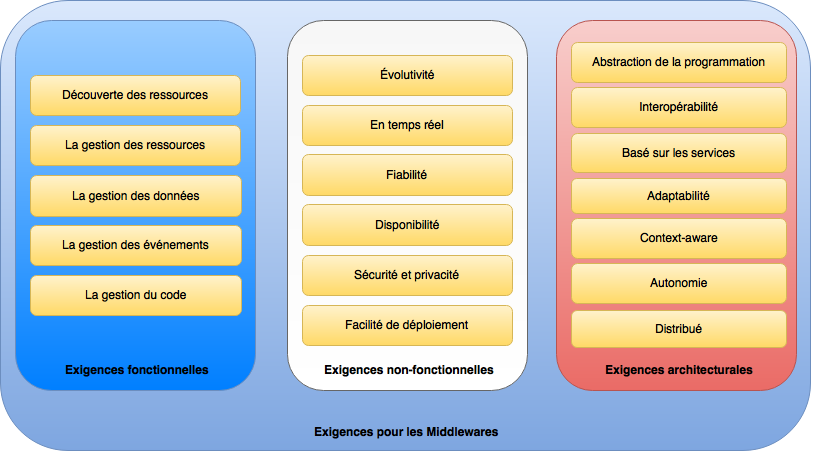
\includegraphics[width=1.1\textwidth]{Figure3.png}
	\caption{Protocoles de Communication et Réseaux de notre Système}
	\label{fig:balance}
\end{figure}

Nous avons commencé par l’évaluation de différents protocoles physiques de communication, correspondant aux couches 1 (physique) et 2 (liaison) du modèle standard OSI. Le tableau 1 résume les caractéristiques de ces protocoles (et les met donc en comparaison).

\begin{center}
	\begin{table}[h]
		\hspace{-1.5cm} 
		\begin{tabular}{|c|c|c|c|c|c|c|c|}
		\hline
		Number of Threads & 1 & 2 & 4 & 8 & 16 & 32 & 64 \\ \hline
		\hline
		MySQL Cluster     & 25.11756 & 13.00766 & 6.86814 & 4.17984 & 5.1518  & 5.7257  & 15.40208  \\ \hline
		MySQL Standalone  & 3.22312  & 2.3859   & 1.777   & 1.515   & 1.41776 & 1.45096 & 1.51372   \\ \hline
	\end{tabular}
	\caption{Average Execution Time with Number Max of Requests = 1000, in seconds}
	\end{table}
\end{center}

L’utilisation de nombreux capteurs, sur un patient susceptible de bouger à la fois dans son lit voire dans la pièce nous impose d’office l’utilisation de protocoles sans fils, pour que la mobilité de la personne ne soit pas un problème. Les différents protocoles sans fil existants sont décrits ci-dessous.

Le WiFi (Wireless Fidelity), normalisé sous la forme IEEE 802.11 permet la communication sans fil des différents composants dans des réseaux ad-hocs ou plus centralisés, suivant le protocole IP. Cependant, le WiFi soulève un certain nombre de problèmes, le plus important étant la dépense énergétique pour la transmission, qui n’est pas supportable pour de petits capteurs.

Le Bluetooth, normalisé IEEE 802.15.1, est également un protocole de communication sans fil possible, mais présente certains inconvénients majeurs : la dépense énergétique associée à la transmission, là aussi peu supportable pour de petits capteurs, et ses limitations intrinsèques (un périphérique maître Bluetooth ne peut avoir que 7 périphériques esclaves) ne lui donnent pas la propriété de scalabilité recherchée dans IoT, où le nombre de capteurs peut augmenter fortement. Nous l’avons donc exclu.

Une fois exclu ces protocoles trop consommateurs en énergie, nous avons conservé trois protocoles sans fil majeurs.

La transmission radio-fréquence (IEEE 802.15.4) est une possibilité, relativement peu coûteuse en énergie, propose un faible débit (de 20 à 250 kbit/s) et un mécanisme d’évitement des collisions lors de la transmission. Par ailleurs, la faible portée des émissions (de 10 à 25 m) est intéressante dans une optique de réseau très localisé (autour du lit du patient) s’appuyant sur un point central. Par ailleurs le protocole IEEE 802.15.4 propose un mécanisme d’allocation automatique d’adresse de 16 ou 64 bits, ce qui est pratique pour offrir une flexibilité d’adressage avec un nombre de capteurs variable.

Le Bluetooth Low Energy (BLE) est une variante du Bluetooth offrant des débits raisonnables tout en pouvant fonctionner sur des appareils de faible puissance et avec une faible batterie. Par ailleurs, BLE revient sur certaines limitations du Bluetooth comme le nombre de noeuds pouvant être connectés à un même appareil. Cette limite passe de 7 à lus de 65 000, ce qui laisse une marge appréciable pour des réseaux de capteurs. Un inconvénient à ce système est sa non compatibilité avec des appareils Bluetooth standard.

RFID est un protocole et un appareil sans fil à faible porté qui peut être ajouté à n’importe quel appareil pour le rendre “intelligent”. On peut alors interagir avec ces objets via un lecteur RFID, qui peut généralement également écrire. L’avantage principal de ce système est que la puce RFID n’a absolument pas besoin d’une source d’énergie. L’énergie nécessaire à la lecture est fournie par les ondes provenant du lecteur.

Le protocole Zigbee se base sur des ondes radios (norme IEEE 802.15.4), est à basse consommation d’énergie et permet une communication à courte distance, comme Bluetooth mais de manière moins complexe et moins cher.

Enfin, NFC se base sur un mélange entre RFID et BLE. NFC peut être couplé avec un système d’authentification renforcé pour offrir une plus grande sécurité d’accès, tout en permettant la lecture de ses informations comme on pourrait le faire pour une puce RFID classique. Cependant son inconvénient principal est la portée de lecture, qui impliquerait de “coller” le lecteur à l’appareil comportant la puce NFC.
\\

En se basant sur ce comparatif, nous avons choisi pour le système de notre Smart Hôpital d’éliminer certains protocoles : WiFi et Bluetooth pour des raisons énergétiques, NFC pour des raisons de portée et Zigbee. Nous avons également choisi, dans un soucis de laisser une bonne diversité de capteurs possibles, que notre système de Smart Hôpital pourrait gérer différents protocoles parmi les plus répandus : IEEE 802.15.4 (radio), BLE et RFID, qui sont tous les trois prometteurs vis-à-vis des restrictions des capteurs, tout en offrant un certain nombre de mécanismes de sécurité (particulièrement BLE).
\\

Après avoir étudié les protocoles physiques, intéressons nous aux protocoles de la couche 3.

Le protocole classique de la couche 3 est bien entendu le protocole IP. IPv4 n’est pas envisageable pour l’IoT, en raison du manque d’adresses disponibles par rapport à la quantité croissante d’objets à connecter, et donc à adresser. IPv6, résout ce problème, avec un nombre d’adresses virtuellement illimité, et représente un protocole éprouvé et adapté à de nouvelles problématiques. Cependant, les besoins d’IPv6 en calcul et en stockage, notamment du fait de ses différents entêtes le rend inutilisable en tant que tel sur de nombreux capteurs.

Face à l’IPv6 classique, une alternative a été développée afin de tenir compte de ressources limitées des différents capteurs utilisés sur IoT, mais également des possibilités de transmission limitée de certains protocoles, comme IEEE 802.15.4 dont les trames sont beaucoup plus petites que celles d’IPv6. Cette alternative est 6LoWPAN (IPv6 over Low-Power Wireless Personal Area Network), un protocole venant au dessus d’IEEE 802.15.4 consistant en une simplification d’IPv6 par la diminution des entêtes nécessaires (toutes celles pouvant être déduites par le contexte ne sont pas transmises), et une meilleure gestion de la fragmentation des trames IPv6 par les protocoles de la couche inférieure. Ceci le rend utilisable sur des capteurs qui ne pourraient pas autrement utiliser IPv6. Par ailleurs, la diminution du stockage et du calcul nécessaire entraîne également une baisse du coût énergétique de transmission du paquet. Compte tenu de l’utilisation que nous avons prévu des émetteurs et récepteurs radio (IEEE 802.15.4), nous avons retenu ce protocole comme protocole de couche 3.
\\

Enfin, le système que nous concevons est destiné à fonctionner grâce à des applications à la fois pour téléphones ou tablettes, sur des serveurs ou des agrégateurs. Nous aurons donc besoin de prendre en compte la communication au niveau applicatif, c’est à dire la couche 7 du modèle OSI, et de choisir de façon adéquate les protocoles applicatifs utilisés afin de simplifier le travail de développement des applications.

Dans la littérature académique sur IoT, un certain nombre de protocoles ont été proposés. Nous nous intéresserons ici à trois protocoles particuliers, XMPP, MQTT et enfin Constraint Application Protocol (CoAP).

XMPP est un protocole ouvert permettant l’échange de messages. Présenté comme un protocole phare de l’IoT, il permet un adressage simple des capteurs, via une adresse proche des adresses mail. Une de ses forces est la présence d’un mécanisme de type “Publish-Subscribe”, c’est à dire un mécanisme où une application intéressée s’enregistre (subscribe) auprès du capteur (publisher) afin d’être notifiée lorsque la valeur du capteur évolue. Ceci permet de limiter la bande passante utilisée, par rapport à un envoi périodique des informations. Un de ses inconvénients est sa faible utilisation dans des exemples concrets de systèmes, par exemple au niveau académique.

MQTT (Message Queue Telemetry Transport) est un autre protocole applicatif offrant un mécanisme de type publish-subscribe. Il gère également la communication Machine to Machine, mais est là aussi assez peu présent dans la littérature.

Constraint Application Protocol (CoAP) est un protocole applicatif qui possède de nombreux points communs avec HTTP, bien qu’étant bien plus léger. En particulier, il supporte l’adressage des capteurs et appareils par une adresse de type URI, et il fonctionne sur un système de requêtes/réponses, supportant comme HTTP quatre méthodes de requêtes : GET, PUT, POST et DELETE. Ces deux caractéristiques facilitent l’utilisation d’API de type REST (fréquentes dans les applications mobiles), et la traduction de HTTP vers CoAP et inversement. De plus, CoAP permet de préciser un type de données transmis, comme le type MIME avec HTTP, ce qui facilite la connaissance du contexte et améliore la sémantique des données transmises. Enfin, CoAP est peu exigeant en capacité de stockage et en énergie, est efficace grâce à des entêtes réduites (meilleur ratio de charge utile), et, pouvant s’appuyer sur UDP et DTLS, permet une sécurisation des données.

Compte tenus de ces avantages nombreux, et de l’idée que nous nous faisons de la façon dont les médecins et personnels hospitaliers pourront utiliser des applications pour smartphones ou tablettes, nous avons donc choisi CoAP pour la communication applicative avec nos capteurs.


\section{ Conclusion }
 

\bibliographystyle{unsrt}




\bibliography{references}




\end{document}
